\section{Ring detection}

we are facing deficulties
(1) fuzzy rings.
(2) non-uniform contrast and  brightness
To evaluate the We need to quantify the signal

Hough transform.
common strategy is to apply an edge detection before HT.
Images of micro particles are fuzzy, does not have a crisp edges. 
Signals can be very close to the background.
We imporve the contrast to gain higher SNR instead of edge detection.

\begin{figure}
\centering
\includegraphics[width=0.35\textwidth]{figs/img0-inverse.png}
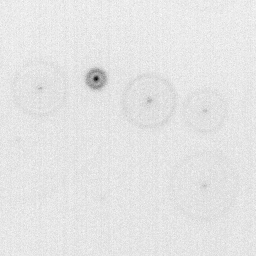
\includegraphics[width=0.35\textwidth]{figs/img0-crop.png}
\end{figure}


contrast, histogram, singmoid, background fitting

\begin{figure}
\centering
\includegraphics[width=0.25\textwidth]{./figs/img0-crop-contrast.png}
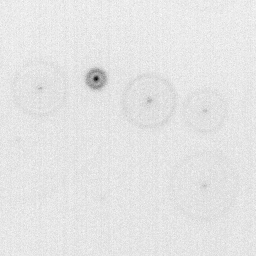
\includegraphics[width=0.35\textwidth]{figs/img0-crop.png}
\end{figure}


